% Figure 4
\ffigbox[\FBwidth]{
\caption{\centering Hypercube \(Q_4\)\\Noeuds non précisés pour la clareté}\label{Fig:qd4}
}{
    \fbox{
        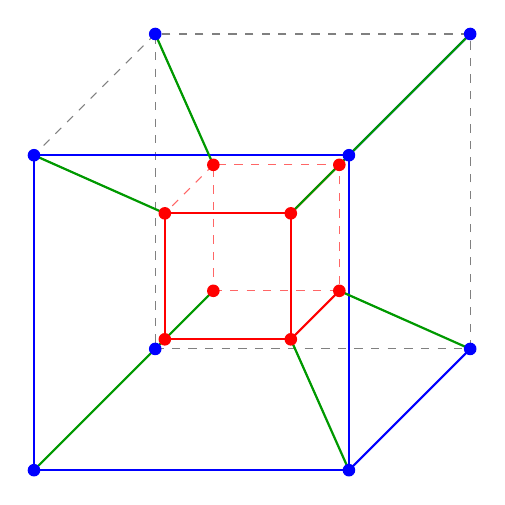
\begin{tikzpicture}[scale=2, line join=round]
            % Define the vertices of the outer cube
            \coordinate (A1) at (0,0,0);
            \coordinate (B1) at (2,0,0);
            \coordinate (C1) at (2,2,0);
            \coordinate (D1) at (0,2,0);
            \coordinate (E1) at (0,0,2);
            \coordinate (F1) at (2,0,2);
            \coordinate (G1) at (2,2,2);
            \coordinate (H1) at (0,2,2);
            
            % Define the vertices of the inner cube (offset)
            \coordinate (A2) at (0.6,0.6,0.6);
            \coordinate (B2) at (1.4,0.6,0.6);
            \coordinate (C2) at (1.4,1.4,0.6);
            \coordinate (D2) at (0.6,1.4,0.6);
            \coordinate (E2) at (0.6,0.6,1.4);
            \coordinate (F2) at (1.4,0.6,1.4);
            \coordinate (G2) at (1.4,1.4,1.4);
            \coordinate (H2) at (0.6,1.4,1.4);
            
            % Draw the outer cube (hidden edges dashed)
            \draw[dashed, gray] (A1) -- (B1) -- (C1) -- (D1) -- cycle; % bottom face
            \draw[dashed, gray] (A1) -- (E1);
            \draw[dashed, gray] (D1) -- (H1);
            \draw[blue, thick] (B1) -- (F1);
            \draw[blue, thick] (C1) -- (G1);
            \draw[blue, thick] (E1) -- (F1) -- (G1) -- (H1) -- cycle; % top face
            
            % Draw the inner cube (hidden edges dashed)
            \draw[dashed, red!60] (A2) -- (B2) -- (C2) -- (D2) -- cycle; % bottom face
            \draw[dashed, red!60] (A2) -- (E2);
            \draw[dashed, red!60] (D2) -- (H2);
            \draw[red, thick] (B2) -- (F2);
            \draw[red, thick] (C2) -- (G2);
            \draw[red, thick] (E2) -- (F2) -- (G2) -- (H2) -- cycle; % top face
            
            % Draw connecting edges between outer and inner cubes (tesseract edges)
            \draw[green!60!black, thick] (A1) -- (A2);
            \draw[green!60!black, thick] (B1) -- (B2);
            \draw[green!60!black, thick] (C1) -- (C2);
            \draw[green!60!black, thick] (D1) -- (D2);
            \draw[green!60!black, thick] (E1) -- (E2);
            \draw[green!60!black, thick] (F1) -- (F2);
            \draw[green!60!black, thick] (G1) -- (G2);
            \draw[green!60!black, thick] (H1) -- (H2);
            
            % Add small dots at vertices for clarity
            \foreach \point in {A1,B1,C1,D1,E1,F1,G1,H1}
                \fill[blue] (\point) circle (0.04);
            \foreach \point in {A2,B2,C2,D2,E2,F2,G2,H2}
                \fill[red] (\point) circle (0.04);
        \end{tikzpicture}
    }
}